%!TEX program = Xelatex
\documentclass{article}
%\usepackage{ctex}
\usepackage{amsmath,amscd,amsbsy,amssymb,latexsym,url,bm,amsthm}
\usepackage{epsfig,graphicx,subfigure}
\usepackage{enumitem,balance,mathtools}
\usepackage{wrapfig}
\usepackage{mathrsfs, euscript}
\usepackage[usenames]{xcolor}
\usepackage{hyperref}
\usepackage{caption}
%\usepackage{subcaption}
\usepackage{float}
\usepackage{listings}
%\usepackage{enumerate}
%\usepackage{algorithm}
%\usepackage{algorithmic}
%\usepackage[vlined,ruled,commentsnumbered,linesnumbered]{algorithm2e}
\usepackage{algorithm}  
\usepackage{algorithmicx}  
\usepackage{algpseudocode}
\usepackage{geometry}
\usepackage{setspace}

\geometry{a4paper,left=2cm,right=2cm,top=2cm,bottom=2cm}

\newtheorem{theorem}{Theorem}[section]
\newtheorem{lemma}[theorem]{Lemma}
\newtheorem{proposition}[theorem]{Proposition}
\newtheorem{corollary}[theorem]{Corollary}
\newtheorem{exercise}{Exercise}[section]
\newtheorem*{solution}{Solution}

\renewcommand{\thefootnote}{\fnsymbol{footnote}}

\newcommand{\postscript}[2]
    {\setlength{\epsfxsize}{#2\hsize}
    \centerline{\epsfbox{#1}}}

\renewcommand{\baselinestretch}{1.0}

\usepackage{url}

\title{Report For CS385 Personal Project}
\author{Yanming Liu; ID: 518030910393}

\begin{document}

\maketitle
\noindent\textbf{Declare} \\
All the code in this project is written by myself, and you can check it : \url{https://github.com/lym01803/CS385_Project1}, which is 
my personal repository. I only use third-party libraries for the following: 
\begin{itemize}
    \item Visualization, e.g. PCA, t-SNE, draw curve and histogram.
    \item SVM.
    \item HOG feature.
    \item For CNN model. The network is built by myself. But I use API for network layers, e.g. Conv, BN.
    \item Basic matrix operations. For simple models, I only use pytorch to do simple matrix operations on cuda. I do not use any advanced API, such as 
    built-in network layers, optimizers and auto-gradient. In fact, to confirm it, I set the requires\_grad attribute of tensors to False.
\end{itemize}
\textbf{Note}\\
During the project, I discussed and exchanged opinions with my classmates many times. In the analysis of logistic regression model, my opinion may 
be similar to that of my classmate Yuxuan Xiong. Please note that if there are some similarities in our analysis, it is the result of our discussion, not plagiarism.

\section{Introduction}
In this project, I do the following things:
\begin{itemize}
    \item Processed the data set;
    \item Implement several basic models: Logistic Regression, LDA, kernel based Logistic Regression, SVM and CNN;
    \item Try two regular terms: Ridge and Lasso;
    \item Visualization: HOG feature, CNN feature and distribution of LDA and Logistic Regression;
    \item Analysis: mainly about the logistic regression. 
\end{itemize}

In fact, the models in this project are all discriminative models, and they are all closely related to logistic regression: LDA and logistic regression have different goals, but they take the same way to solve 
the discrimination problem: learning a projection direction to separate data; The motivation of the SVM model comes from the discussion of the margin in linear binary discrimination problem; The kernel is an extension 
of the linear model to the nonlinear model, which is equivalent to a linear model for high-dimensional (probably non-linear) features $\phi(X)$; CNN can be regarded as using a learnable deep network to produce the features 
of input images instead of using the manual designed HOG features, which is essentially a binary classifier (logistic regression) or a multi-classifier (extension of logistic regression, sigmoid -> softmax) of the CNN based features. 
Therefore, in the subsequent analysis of the project, the discussion will mainly focus on a basic point, the linear logistic regression model. 

\section{Data Process}
\subsection{Crop and Padding}
The given data set has two format: 1. original images with character level bounding boxes; 2. The cropped images. 

Since the borders of digits are usually not square, the square cropped images mostly contain part of other digits. Although someone says 
that such noise does not affect the performance of the classifier (most likely because the translation invariance of HOG is not good), I still do not plan to use it. 

Therefore, I crop the original images by myself according to the given digit boxes, then padding the images into squares symmetrically, and then resize them to a size of $32\times 32$.
For the color to padding, I choose the average color of the border pixels of cropped images (averaged for each channel). I am not sure if such an operation meets the specifications of the CV field, 
but at least the images obtained in this way seems to be of high quality to my eyes and is suitable for training discriminative models, I think.

The comparison between the two official offered data and the data processed by myself is shown in the followed Fig. \ref{datasetimage}.

\begin{figure}[H]
    \centering
    \begin{minipage}{0.32\textwidth}
        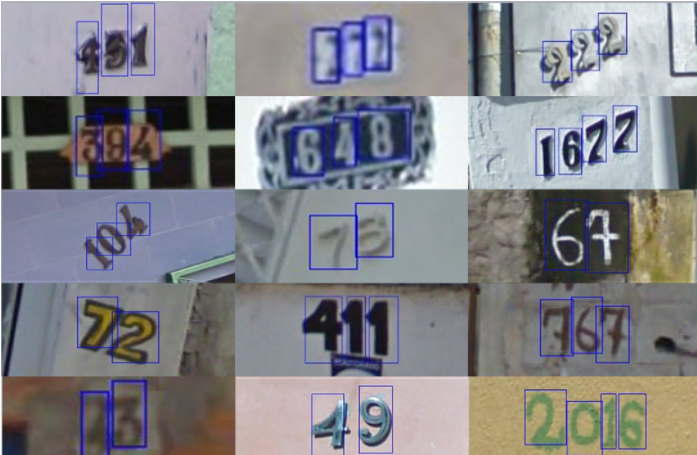
\includegraphics[width=0.95\textwidth]{fig/1.png}
        Format 1: original images
    \end{minipage}
    \begin{minipage}{0.32\textwidth}
        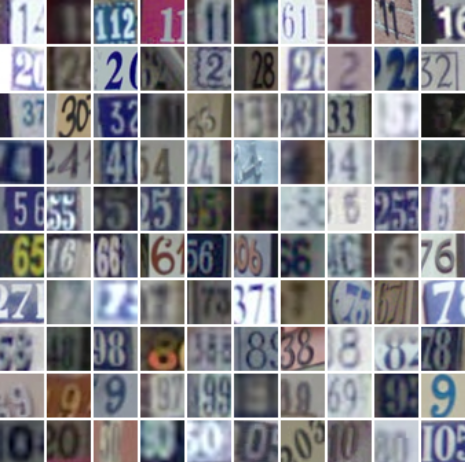
\includegraphics[width=0.95\textwidth]{fig/2.png}
        Format 2: cropped images
    \end{minipage}
    \begin{minipage}{0.32\textwidth}
        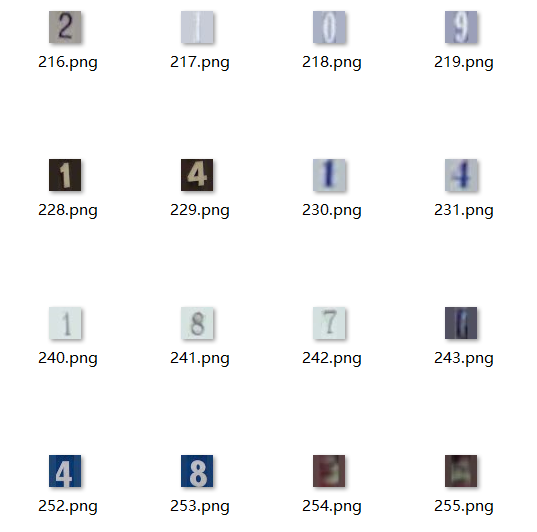
\includegraphics[width=0.95\textwidth]{fig/3.png}
        Images cropped and paddinged by myself
    \end{minipage}
    \caption{Comparison between official data and data processed by myself}
    \label{datasetimage}
\end{figure}
\subsection{HOG Feature}
General experience tells us that directly using the three-channel pixels of an image as the input features may not be effective. It is usually believed that the local gradient (both norm and direction) of an image can 
reflect image features such as object edges and textures. Therefore, the HOG feature of the image is used as the input of models (except CNN) here. A third-party library cv2.HOGDescriptor is used here. The parameters are 
shown in the following Table \ref{hogparam}, and finally $1764$-dimensional feature vectors are obtained.
\begin{table}[H]
    \centering
    \caption{The HOG parameters setting}
    \label{hogparam}
    \begin{tabular}{|lr|lr|}
        \hline
        input size& $32\times 32\times 3$&window size&$32\times 32$\\
        block size& $8\times 8$&block stride& $4\times 4$\\
        cell size & $4\times 4$& bin & 9\\
        \hline
    \end{tabular}
\end{table}

\section{Logistic Regression}
\subsection{Implement}
I follow eq. \ref{eq1}.
\begin{spacing}{1.5}
\begin{equation}
    \begin{array}{rl}
        L_i &= y_i\log p_i + (1-y_i)\log (1-p_i)\\
            &= y_iX_i^\top \beta - \log(1+\exp(X_i^\top \beta))\\
        \dfrac{\partial}{\partial\beta}L_i &= 
        y_iX_i - \dfrac{\exp(X_i^\top\beta)}{1+\exp(X_i^\top\beta)}\cdot X_i\\
            &= (y_i - p_i)\cdot X_i
    \end{array}
    \label{eq1}
\end{equation}
\end{spacing}
For efficient calculation, I do not calculate the loss $L_i$ in the program. Instead I directly calculate the gradient $\partial L_i/\partial\beta$ and perform gradient descent.  

For prediction, typical logistic regression is a bianry discriminative model, so for the 10-classes discrimination problem, I use 10 independent logistic regression models. The $i-$th ($0\leq i \leq 9$) model predict the 
probability $Pr(y = i| X, \beta_i)$. So predicted class is calculated by $\mathtt{predict}=\arg\max_{0\leq i\leq 9} Pr(y=i|X, \beta_i)$.

\subsection{Result}
Because 10 independent binary discriminative models are used here, and the result of argmax is used as the final predicted value, the model evaluation indicators here are shown as follows:
\begin{itemize}
    \item Evaluate the performance of the logistic regression model: the accuracy of a single logistic regression model on their respective binary discrimination tasks.
    \item Evaluate the performance of the multi-discrimination model composed of 10 binary discriminator: 
    \begin{itemize}
        \item Evaluate the recall rate corresponding to each digit.
        \item Evaluate the overall accuracy of the model on the multi-discrimination task.
    \end{itemize}
\end{itemize}
The experiment settings are shown in the Table \ref{setting}: \textbf{Note} Here all parameters tuning are in order to study the model, not to improve the score on test set, so there is no need to set a validation set.
\begin{table}[H]
    \centering
    \caption{Experiment Settings}
    \label{setting}
    \begin{tabular}{|c|c|}
        \hline
        Train Data & 73257 images from train folder\\
        Test Data & 26032 images from test folder\\
        Learing Rate & 1.0, 0.1, 0.01 or 0.001\\
        Ridge Coefficient & 0.1, 0.01, 0.001 or 0\\
        Lasso Coefficient & 0.1 or 0\\
        Epoch & 100\\
        Batch Size & 256\\
        Optimizing Method& SGD or Adam\\
        \hline
    \end{tabular}
\end{table}
\subsubsection{Performance - learning rate}
Use Adam. No Ridge loss or Lasso loss. The result is shown in Table \ref{lracclr}
\begin{table}[H]
    \centering
    \caption {Acc-lr}
    \label {lracclr}
    \begin{tabular}{c|c|c}
        \hline 
        lr & Train Acc & Test Acc\\
        \hline
        1.0 &  0.7902 & 0.7105\\
        1e-1 & 0.8673 & 0.7939 \\
        1e-2 & 0.8716 & 0.8137 \\
        1e-3 & 0.8545 & 0.8175 \\
        \hline
    \end{tabular}
\end{table}
There are more details in Fig. \ref{lracclrfig}.
\begin{figure}[H]
    \centering
    \begin{minipage}{0.48\textwidth}
        \centering
        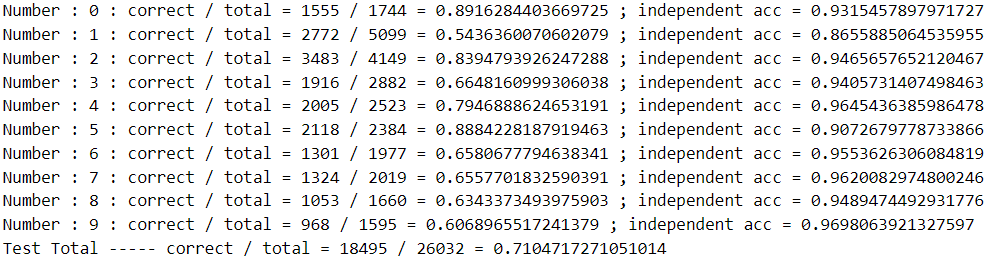
\includegraphics[width=0.95\textwidth]{fig/4-4.png}\\
        lr = 1.0
    \end{minipage}
    \begin{minipage}{0.48\textwidth}
        \centering
        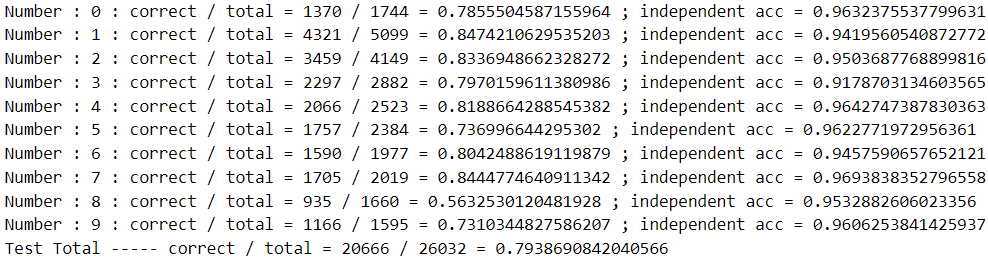
\includegraphics[width=0.95\textwidth]{fig/4-3.png}\\
        lr = 1e-1
    \end{minipage}
    \begin{minipage}{0.48\textwidth}
        \centering
        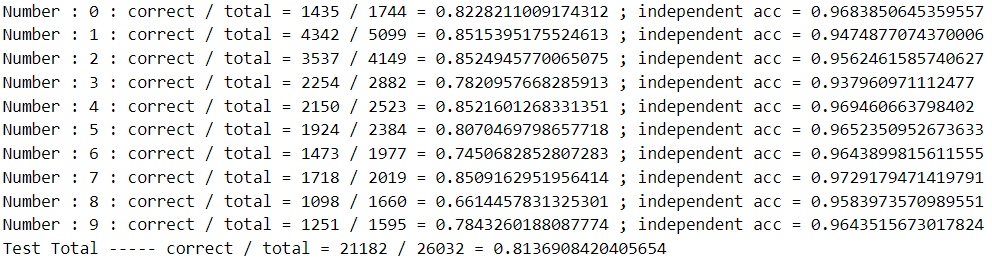
\includegraphics[width=0.95\textwidth]{fig/4-2.png}\\
        lr = 1e-2
    \end{minipage}
    \begin{minipage}{0.48\textwidth}
        \centering
        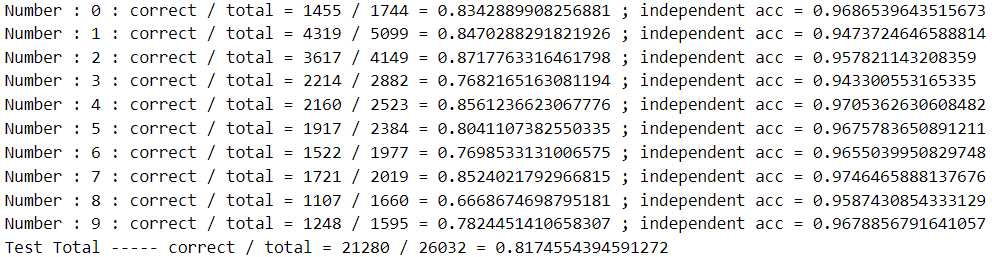
\includegraphics[width=0.95\textwidth]{fig/4-1.png}\\
        lr = 1e-3
    \end{minipage}
    \caption{Acc-lr details}
    \label{lracclrfig}
\end{figure}
Trivial (so I will show as few of these curves as possible later) performance curves are shown in Fig. \ref{performancecurve}.
\begin{figure}[H]
    \centering
    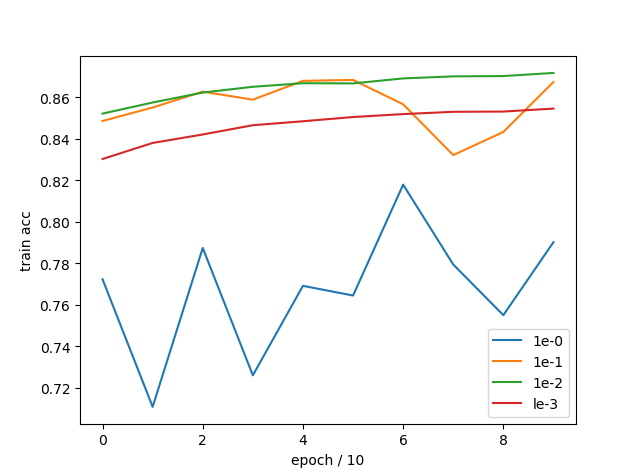
\includegraphics[width=0.5\textwidth]{fig/4-5.png}
    \caption{Performance curves}
    \label{performancecurve}
\end{figure}
\noindent \textbf{Conclusion}: I think it is appropriate to set the learning rate to 1e-2 here.
\subsubsection{Performance - Adam}
No Ridge or Lasso loss. lr = 1e-2. The result is shown in Table \ref{lraccadam}
\begin{table}[H]
    \centering
    \caption {Acc-Adam}
    \label {lraccadam}
    \begin{tabular}{c|c|c|c}
        \hline 
        Optimizer & Train Acc & Test Acc & Running Time\\
        \hline
        SGD & 0.8402 & 0.8105 & about 30 s\\
        Adam & 0.8716 & 0.8137 & about 60 s\\
        \hline
    \end{tabular}
\end{table}
\noindent \textbf{Conclusion}: SGD is a little faster. Adam is better at fitting training data, in other words, its ability to solve the function minimums is stronger. However, there is no significant difference in the performance on the test set.
Therefore, the Optimizer is not a particularly import thing.
\subsubsection{Performance - Ridge / Lasso}
Use Adam. Set lr = 1e-2. The result is shown in Table \ref{ridgelasso}.
\begin{table}[H]
    \centering
    \caption {Performance-Ridge / Lasso}
    \label {ridgelasso}
    \begin{tabular}{c|c|c|c|c|c|c}
        \hline 
        Ridge coef& Lasso coef & Train Acc & Test Acc & Norm1 & Norm2 & Norm1 / Norm2\\
        \hline
        1e-1 & - & 0.8366 & 0.8036 & 160.22 & 5.56 & 28.79\\
        le-2 & - & 0.8548 & 0.8165 & 382.20 & 12.57 & 30.40 \\
        1e-3 & - & 0.8647 & 0.8121 & 865.84 & 26.67 & 32.47 \\
        - & 1e-1 & 0.8222 & 0.7983 & 76.73 & 9.01 & 8.52 \\
        - & 1.0 (decay) * & 0.8638 & 0.8185 & 761.72 & 25.36 & 29.82\\
        \hline
    \end{tabular}
\end{table}
* The decay method : lasso coef start at 1.0, and decay by 0.1 every 20 epochs. This idea is from the Lasso Regression discussed in class. But the above experimental results show that this 
method, decaying during iteration, has no effect \textbf{here}. \\

\noindent\textbf{Conclusion}:
As regular term, Ridge loss and Lasso loss will reduce the fitting performance on the train set. The ability to avoid over-fitting is also limited, at least no significant improvement on test set can be seen from the above experimental results.
Ridge loss can indeed reduce the Norm2 of the parameter ($\beta$ here), but notice that it will also reduce Norm1 at the same time. In fact, when the coef of Ridge takes different values, the values of Norm1 $/$ Norm2 are almost the same. The Lasso loss 
more significantly reduces the train set fitting ability. Lasso loss can reduce both Norm1 and Norm2, but it is worth noting that it can significantly reduce Norm1 / Norm2, which is a quantity that I think can reflect the sparseness of the parameter. 

It also confirms a problem discussed in class. A linear model can perform well on the test set, but this does not necessarily mean that it is a good model. We should pay attention to what the parameters of linear model have learned. In order to prevent the parameters from learning too much 
redundant information, we introduced Lasso. Lasso can reduce Norm1 / Norm2, which means that the parameters are sparser. That is actually what we expect. We do not expect Lasso to significantly improve the performance of model on the test set.

\subsubsection{Distribution of $X^\top\beta$}
This problem is very interesting. I will analysis it later together with LDA.

\section{Linear Discriminant Analysis (LDA)}
\subsection{Implement}
\subsubsection{Train}
Just follow the eq. \ref{ldaeq}:
\begin{spacing}{1.5}
\begin{equation}
    \label{ldaeq}
    \begin{array}{rl}
        S_W =& n^+\Sigma^+ + n^-\Sigma^-\\
        \beta =& S^{-1}_W (\mu^+-\mu^-)
    \end{array}
\end{equation}
\end{spacing}
\subsubsection{Predict}
LDA is originally a visualization tool and is not directly used as a binayr classifier. But considering that, through LDA we can get the projection $X^\top\beta$, and can classify it according to this projection. 
The simplest way is to calculate a threshold to classify. 

However, here we need to construct 10 binary LDA classifiers to do the multi-classify task. That is to say, it is unreasonable to directly predict a 0 or 1 result. Because of the model errors, it is possible that an image is predicted 
as a positive sample in more than one classifiers, which makes it difficult to perform multi-classfication. Therefore, I am here to give an approach based on conditional probability:

We \textbf{assume} that the positive and negative samples of $X\beta$ after the LDA projection respectively obey the normal distribution: $(X^\top\beta)^+\sim N(\mu^+, {\sigma^+}^2)$ and $(X^\top\beta)^-\sim N(\mu^-, {\sigma^-}^2)$. Then we can write the conditional probability :
\begin{spacing}{2.0}
\begin{equation}
    \label{ldapredict}
\begin{array}{rl}
    P(y=+|X^\top\beta)=&\dfrac{P(y=+)\cdot P(X^\top\beta|y=+)}{P(y=+)\cdot P(X^\top\beta|y=+) + P(y=-)\cdot P(X^\top\beta|y=-)}\\
    =&\dfrac{n^+ \cdot \dfrac{1}{\sqrt{2\pi}\sigma^+}\exp\left(-\dfrac{1}{2{\sigma^{+}}^2}(X^\top\beta - \mu^+)^2\right)}{n^+ \cdot \dfrac{1}{\sqrt{2\pi}\sigma^+}\exp\left(-\dfrac{1}{2{\sigma^{+}}^2}(X^\top\beta - \mu^+)^2\right) + n^- \cdot \dfrac{1}{\sqrt{2\pi}\sigma^-}\exp\left(-\dfrac{1}{2{\sigma^{-}}^2}(X^\top\beta - \mu^-)^2\right)}
\end{array}
\end{equation}
\end{spacing}
Follow the eq. \ref{ldapredict}, the predicted value of LDA model is a probability between 0 and 1, and its meaning is the same as the predicted value in logistic regression. In this way, we can use the same approach as the logistic regression to do the multi-classfication task.
\subsection{Result}
\subsubsection{Settings}
Just use the same train and test data set as logistic regression.
\subsubsection{Accuracy}
The result is shown below in Fig. \ref{acclda}:\\
The first 10 lines show the recall rate for each digit. The last line shows the overall accuracy of the multi-classifier.
\begin{figure}[H]
    \centering
    \caption{Acc for LDA}
    \label{acclda}
    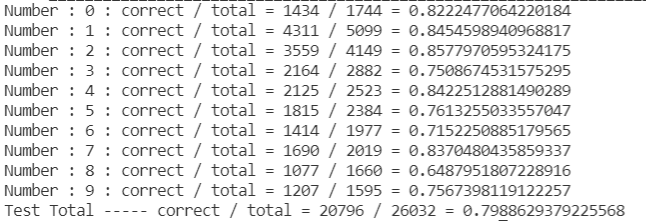
\includegraphics[width=0.6\textwidth]{fig/5-1.png}
\end{figure}
\subsubsection{Distribution of $X^\top\beta$}
\begin{figure}[H]
    \centering
    \begin{minipage}{0.19\textwidth}
        \centering
        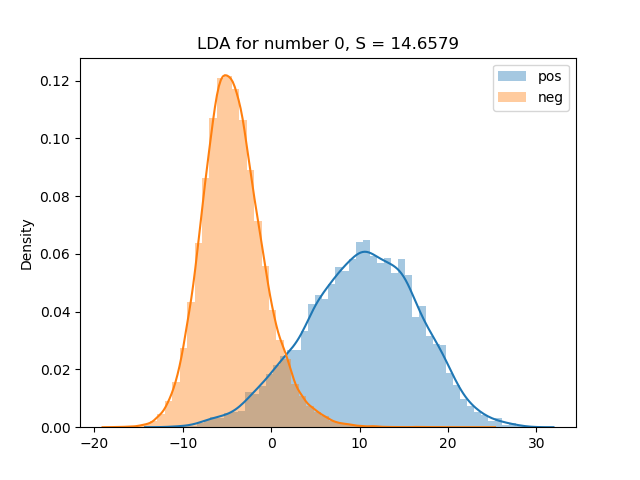
\includegraphics[width=0.95\textwidth]{fig/lda/0.png}
        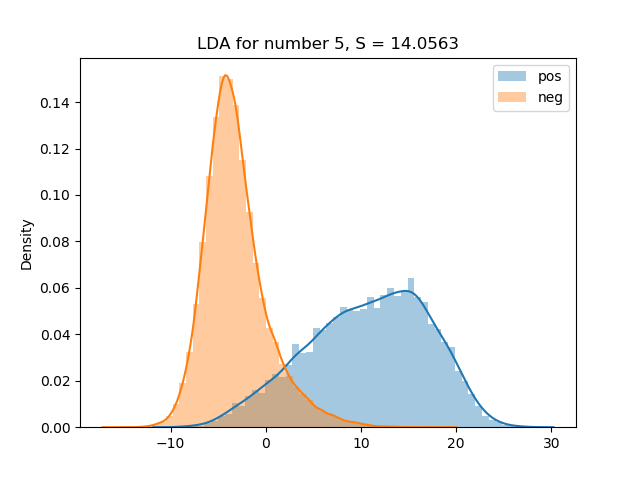
\includegraphics[width=0.95\textwidth]{fig/lda/5.png}
    \end{minipage}
    \begin{minipage}{0.19\textwidth}
        \centering
        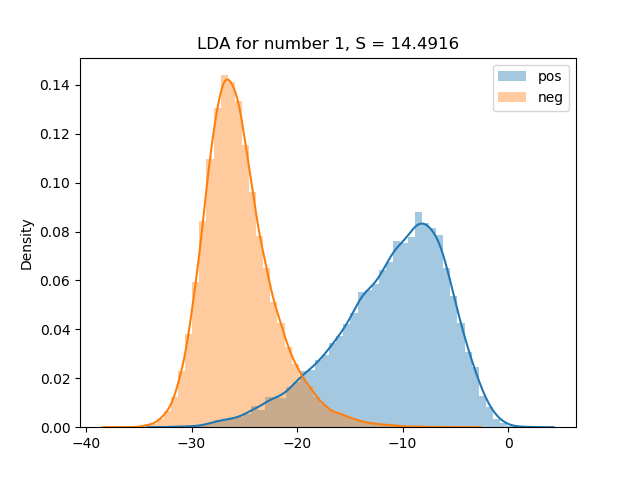
\includegraphics[width=0.95\textwidth]{fig/lda/1.png}
        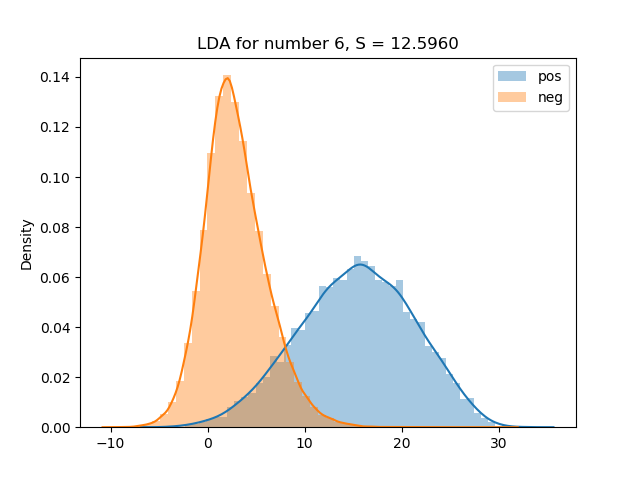
\includegraphics[width=0.95\textwidth]{fig/lda/6.png}
    \end{minipage}
    \begin{minipage}{0.19\textwidth}
        \centering
        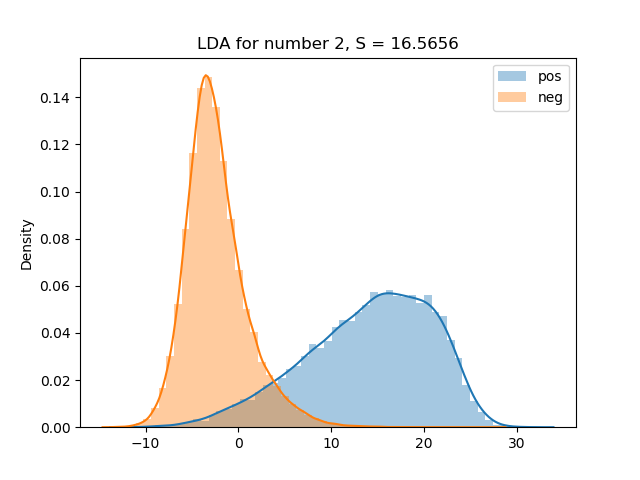
\includegraphics[width=0.95\textwidth]{fig/lda/2.png}
        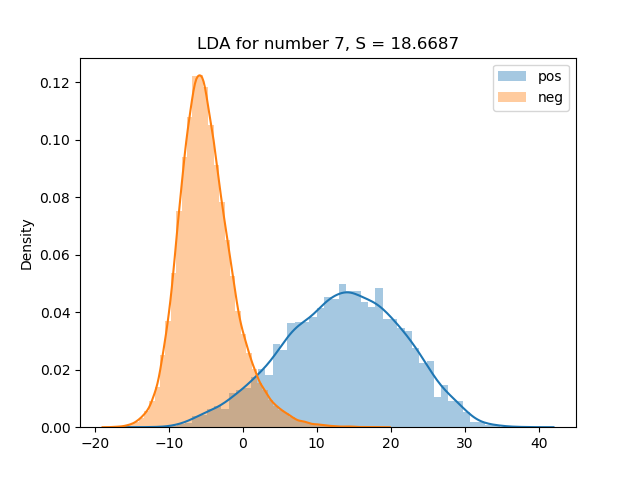
\includegraphics[width=0.95\textwidth]{fig/lda/7.png}
    \end{minipage}
    \begin{minipage}{0.19\textwidth}
        \centering
        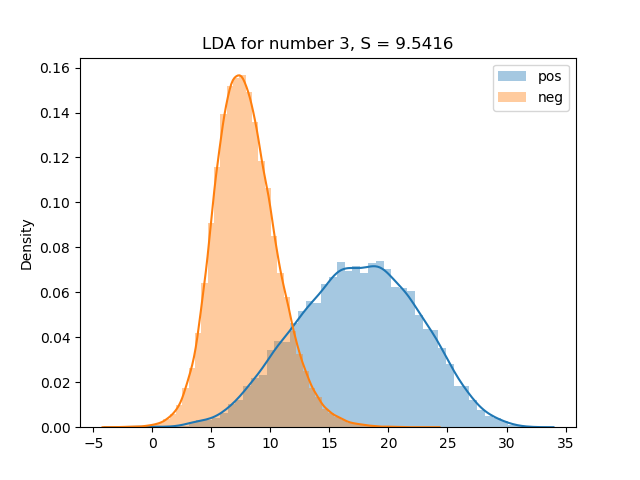
\includegraphics[width=0.95\textwidth]{fig/lda/3.png}
        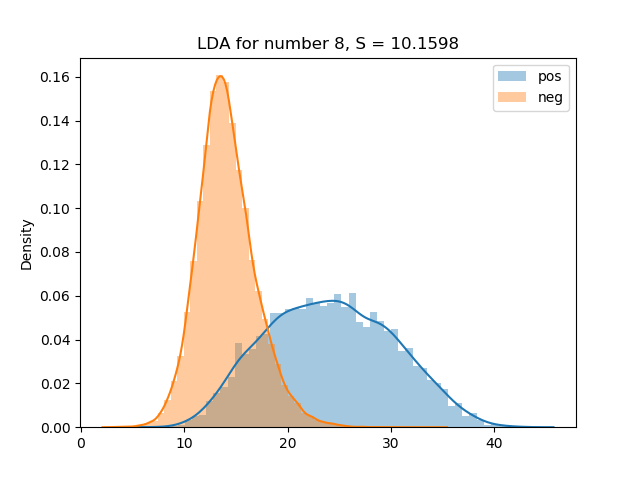
\includegraphics[width=0.95\textwidth]{fig/lda/8.png}
    \end{minipage}
    \begin{minipage}{0.19\textwidth}
        \centering
        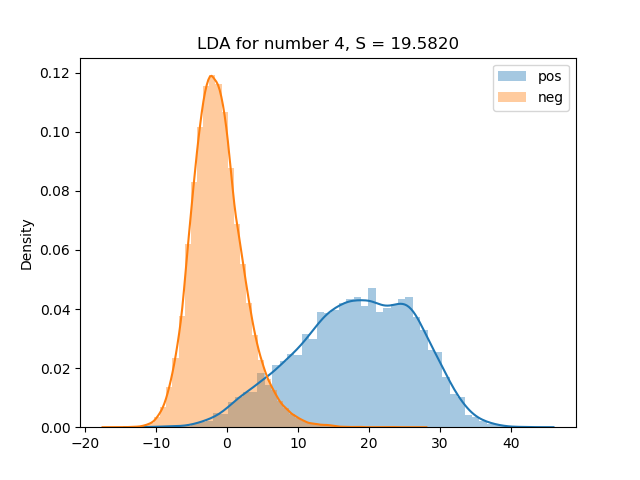
\includegraphics[width=0.95\textwidth]{fig/lda/4.png}
        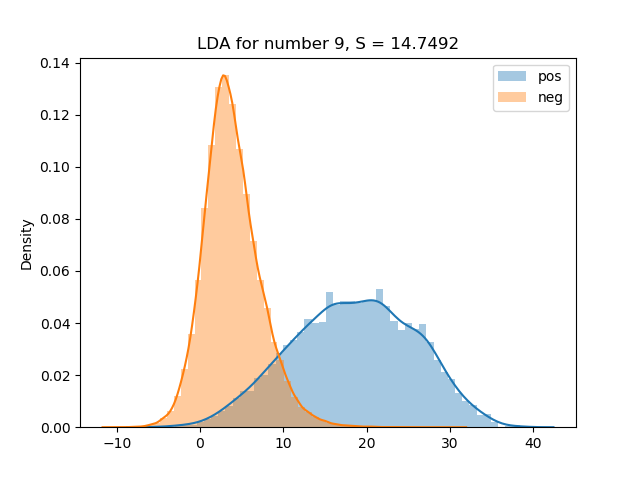
\includegraphics[width=0.95\textwidth]{fig/lda/9.png}
    \end{minipage}
    \caption{Distribution of $X^\top\beta$ for LDA}
\end{figure}
I am interested in what the distribution of $X^\top\beta$ of logistic regression looks like.
\begin{figure}[H]
    \centering
    \begin{minipage}{0.19\textwidth}
        \centering
        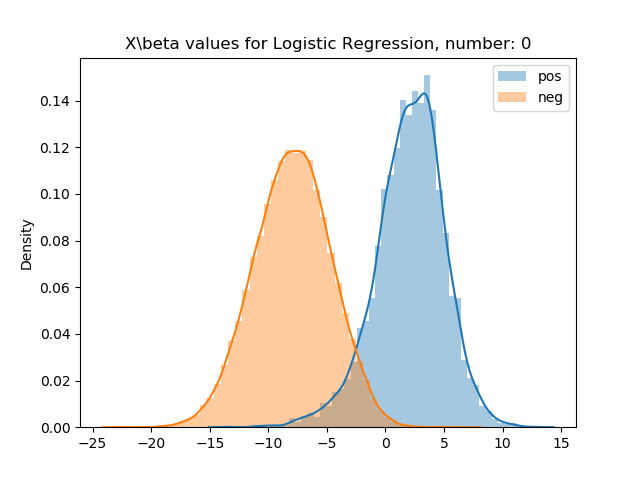
\includegraphics[width=0.95\textwidth]{fig/lr/0.png}
        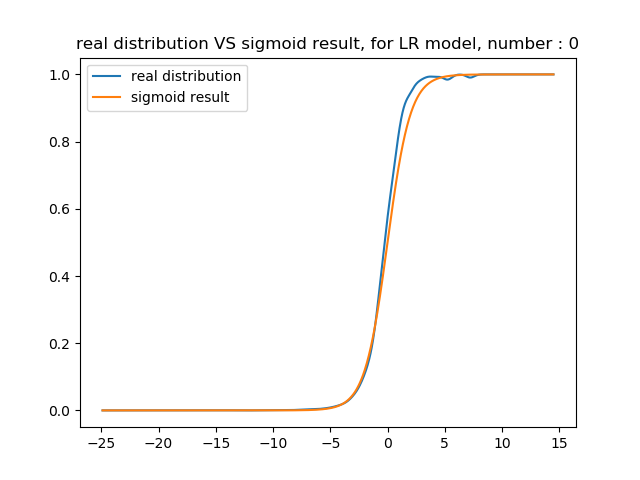
\includegraphics[width=0.95\textwidth]{fig/lr/0-2.png}
        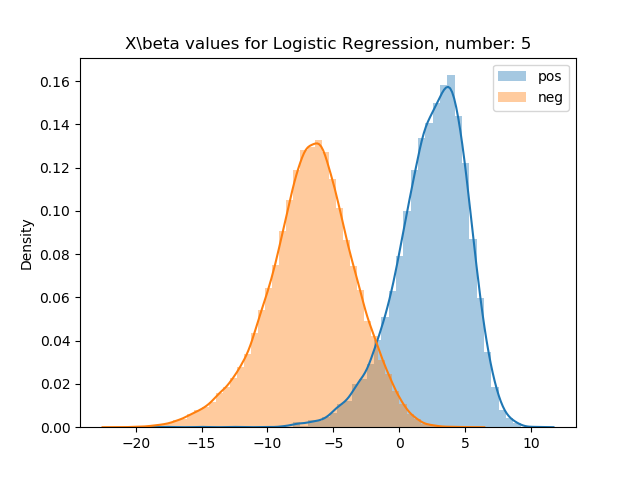
\includegraphics[width=0.95\textwidth]{fig/lr/5.png}
        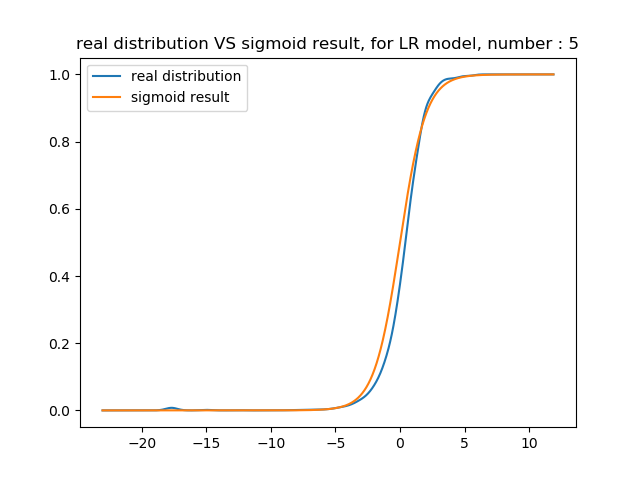
\includegraphics[width=0.95\textwidth]{fig/lr/5-2.png}
    \end{minipage}
    \begin{minipage}{0.19\textwidth}
        \centering
        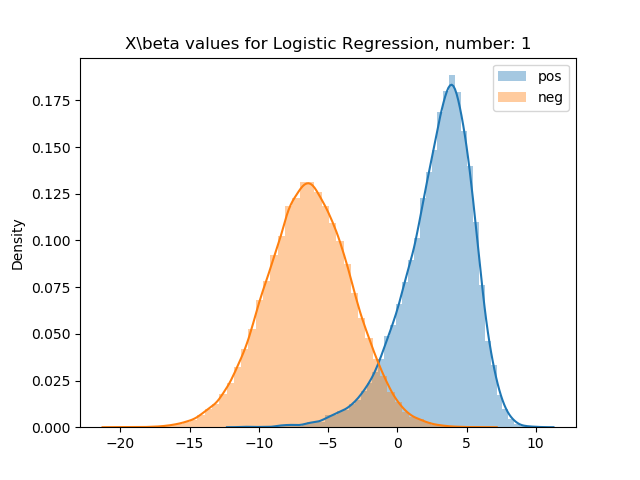
\includegraphics[width=0.95\textwidth]{fig/lr/1.png}
        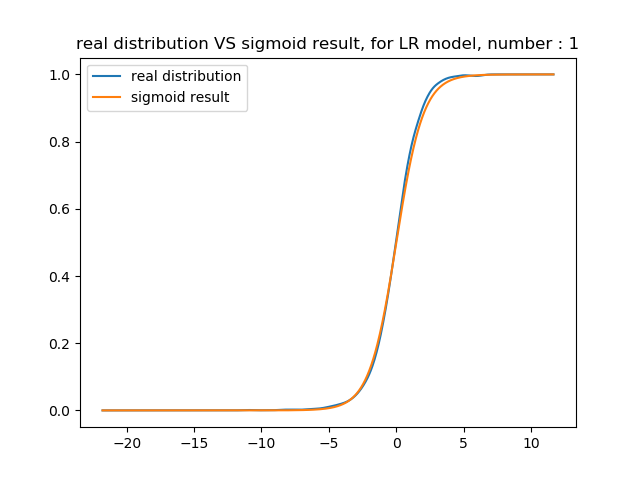
\includegraphics[width=0.95\textwidth]{fig/lr/1-2.png}
        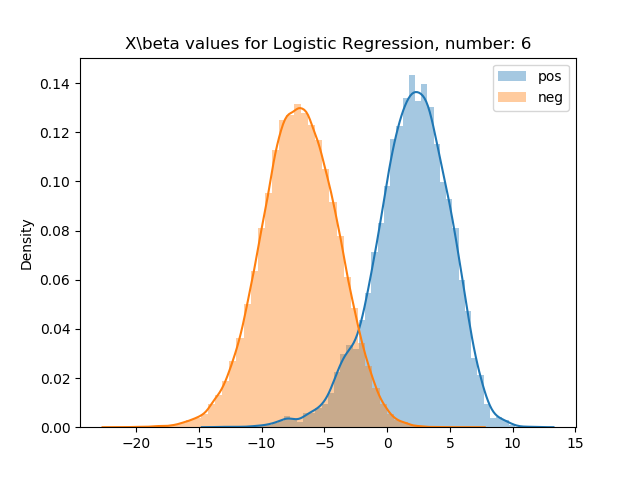
\includegraphics[width=0.95\textwidth]{fig/lr/6.png}
        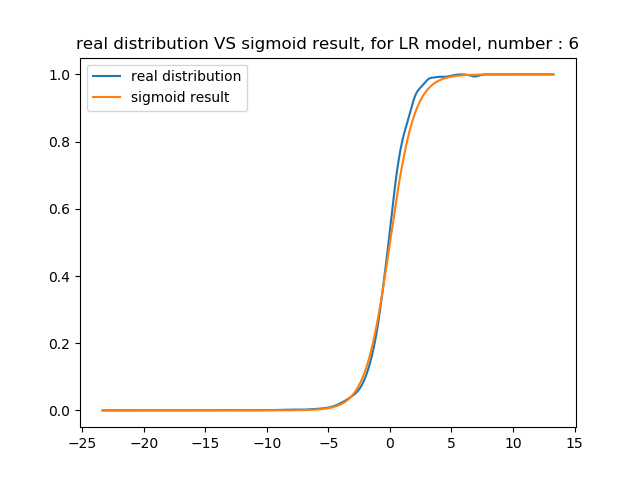
\includegraphics[width=0.95\textwidth]{fig/lr/6-2.png}
    \end{minipage}
    \begin{minipage}{0.19\textwidth}
        \centering
        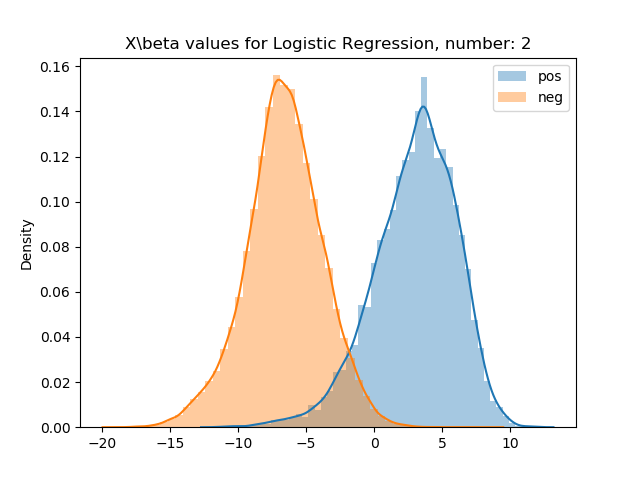
\includegraphics[width=0.95\textwidth]{fig/lr/2.png}
        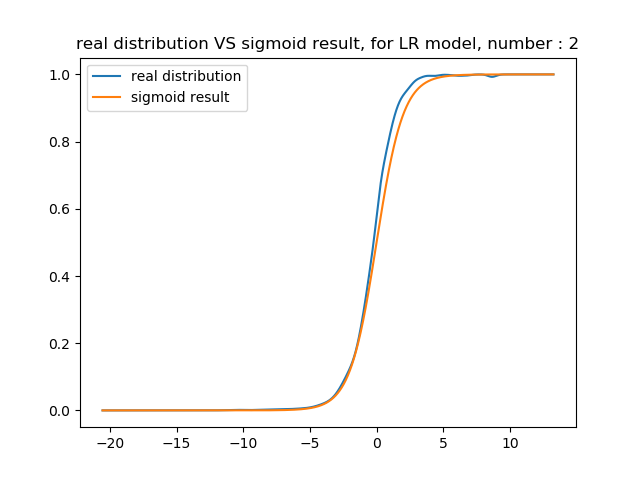
\includegraphics[width=0.95\textwidth]{fig/lr/2-2.png}
        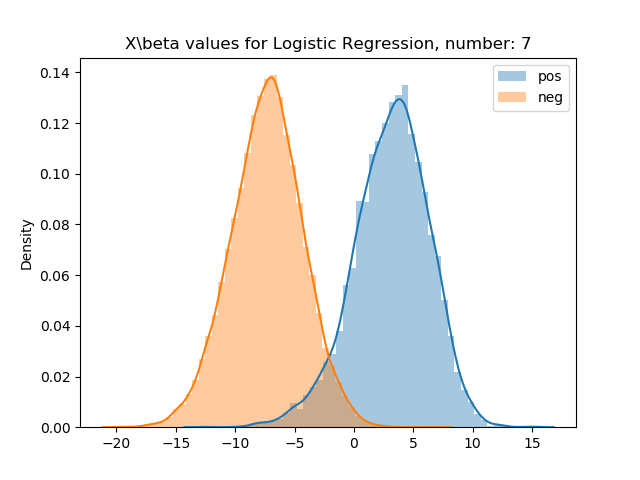
\includegraphics[width=0.95\textwidth]{fig/lr/7.png}
        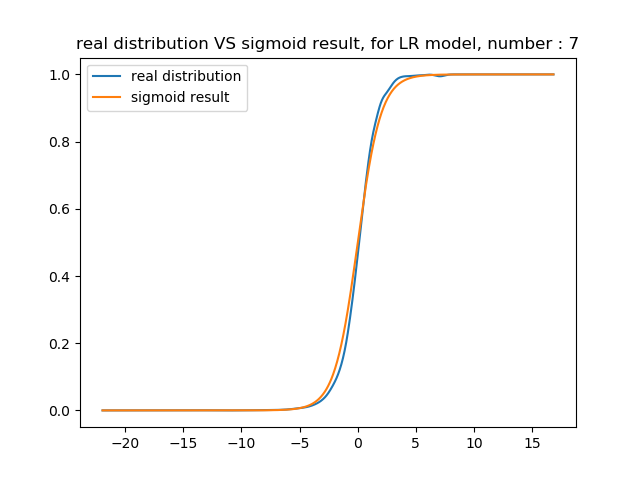
\includegraphics[width=0.95\textwidth]{fig/lr/7-2.png}
    \end{minipage}
    \begin{minipage}{0.19\textwidth}
        \centering
        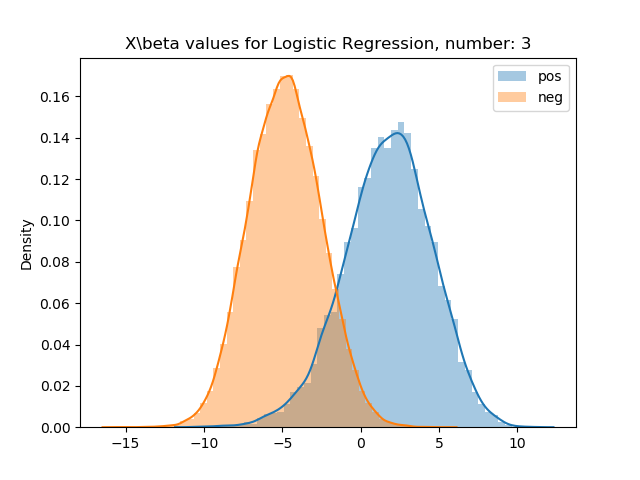
\includegraphics[width=0.95\textwidth]{fig/lr/3.png}
        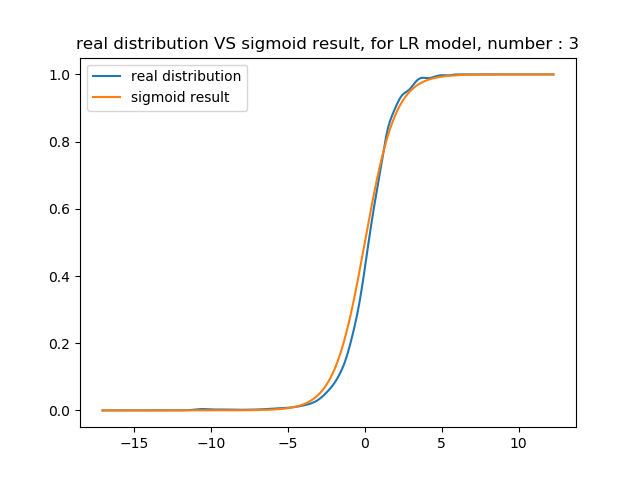
\includegraphics[width=0.95\textwidth]{fig/lr/3-2.png}
        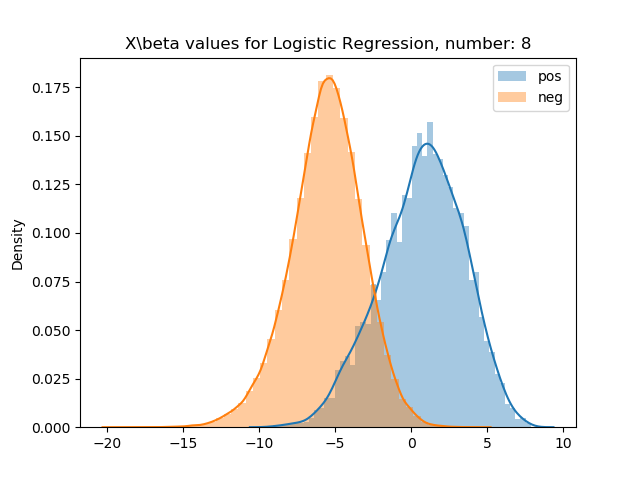
\includegraphics[width=0.95\textwidth]{fig/lr/8.png}
        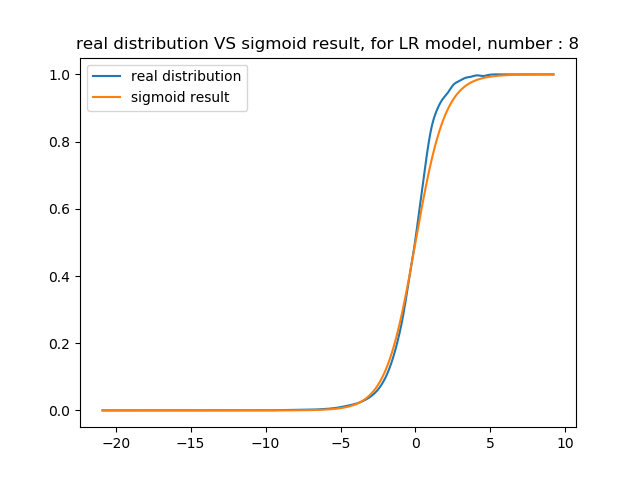
\includegraphics[width=0.95\textwidth]{fig/lr/8-2.png}
    \end{minipage}
    \begin{minipage}{0.19\textwidth}
        \centering
        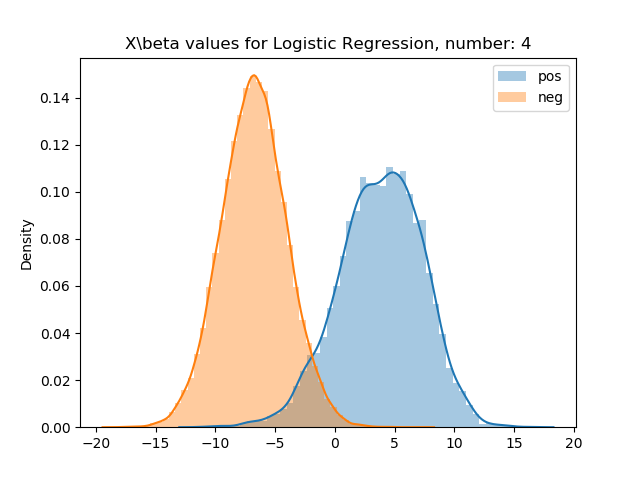
\includegraphics[width=0.95\textwidth]{fig/lr/4.png}
        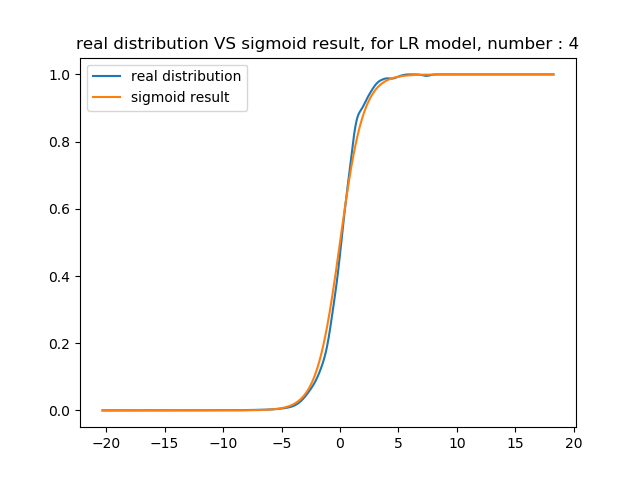
\includegraphics[width=0.95\textwidth]{fig/lr/4-2.png}
        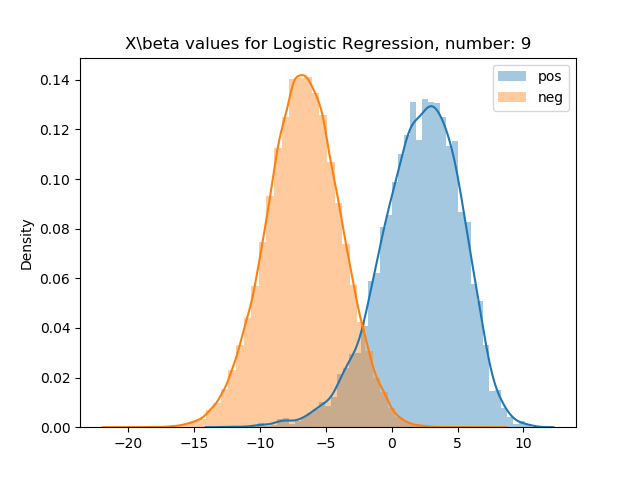
\includegraphics[width=0.95\textwidth]{fig/lr/9.png}
        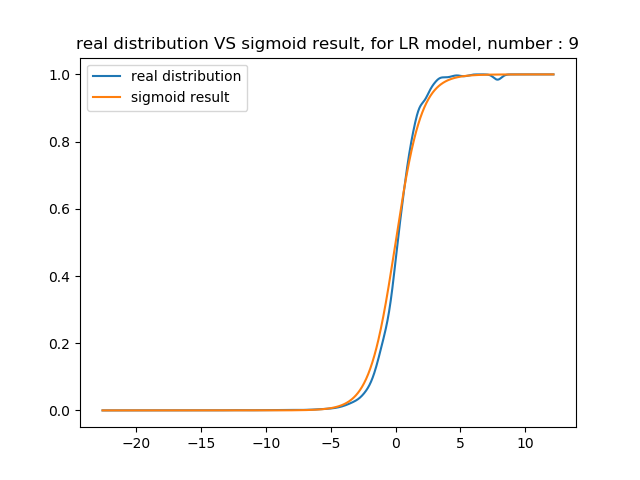
\includegraphics[width=0.95\textwidth]{fig/lr/9-2.png}
    \end{minipage}
    \caption{Distribution of $X^\top\beta$ and $Pr(y=+1|X^\top\beta)$ for LR}
    \label{lrdist}
\end{figure}
Fig. \ref{lrdist} show the distribution of $X^\top\beta$ and $Pr(y=+1|X^\top\beta)$. The figure shows: 
\begin{itemize}
    \item The projection $X^\top\beta$ is close to normal distribution, intuitively.
    \item Projections of LDA and LR are similar, but different.
    \begin{itemize}
        \item LDA learn a projection direction to maximize $S = \dfrac{\sigma^2_{inter}}{\sigma^2_{intra}}$;
        \item LR learn a projection to maximize the likelihood
    \end{itemize} 
    \item LR learn a projection direction to make the conditional probability $f(X^\top\beta)=Pr(y=+1|X^\top\beta)$ close to the sigmoid function $g=\mathtt{sigmoid}(X^\top\beta)$ 
\end{itemize}
Note that there is a logic chain: LR learn a projection direction to make the conditional probability distribution close to sigmoid function. And LR use sigmoid / logistic function. -> If we choose another function, and make the conditional probability 
distribution close to it, then we will get another regression model ! -> The reason why we choose sigmoid function may be that sigmoid function is a reasonable conditional probability distribution. But why? \\

I think I can give an explanation for leftover problem in our class: Why we use logistic function to do logistic regression ? 
Why we use $X^\top\beta = \log\dfrac{p}{1-p}, p=\mathtt{sigmoid}(X^\top\beta)$ ?
\\
\textbf{Explanation}\\
Assume that $Pr(X^\top\beta|y=+)\sim N(\mu_+, \sigma_+^2)$, $Pr(X^\top\beta|y=-)\sim N(\mu_-, \sigma_-^2)$. Why assume a normal distribution? When there is no known condition, if we have to make a assumption, then it is more reasonable to assume it as a normal distribution. And the above visualization of LDA also tells us that 
this distribution is like a normal distribution. Then we can write :
\begin{equation}
    Pr(y=+|X^\top\beta)=\dfrac{Pr(y=+)\cdot \mathtt{const}_1\cdot \exp\left(-\dfrac{1}{2\sigma_+^2}(X^\top\beta-\mu_+)^2\right)}{Pr(y=+)\cdot \mathtt{const}_1\cdot \exp\left(-\dfrac{1}{2\sigma_+^2}(X^\top\beta-\mu_+)^2\right)+Pr(y=-)\cdot \mathtt{const}_2\cdot \exp\left(-\dfrac{1}{2\sigma_-^2}(X^\top\beta-\mu_-)^2\right)}
\end{equation} 
\textbf{Assume} that $\sigma_+ = \sigma_-$, and hence $\mathtt{const}_1 = \mathtt{const}_2$. Why? No reason, just for calculation convenience. Let $\alpha = \dfrac{Pr(y=-)}{Pr(y=+)}$, then we can rewrite it as :
\begin{spacing}{2.0}
\begin{equation}
    \begin{array}{rl}
        Pr(y=+|X^\top\beta)=&\dfrac{\exp\left(-\dfrac{1}{2\sigma^2}(X^\top\beta-\mu_+)^2\right)}{\exp\left(-\dfrac{1}{2\sigma^2}(X^\top\beta-\mu_+)^2\right) + \alpha\cdot\exp\left(-\dfrac{1}{2\sigma^2}(X^\top\beta-\mu_-)^2\right)}\\
        =&\dfrac{1}{1+\exp\left(\log(\alpha) - \dfrac{1}{2\sigma^2}\left(2(\mu_+-\mu_-)X^\top\beta+(\mu_-^2-\mu_+^2)\right)\right)}\\
        =&\dfrac{1}{1+\exp(-(aX^\top\beta+b))} = \mathtt{sigmoid}(aX^\top\beta+b)
    \end{array}
\end{equation}
where $a=\dfrac{\mu_+-\mu_-}{\sigma^2}$, $b=\dfrac{\mu_-^2-\mu_+^2}{2\sigma^2}-\log\alpha$. And $b \approx -\log \alpha$, if we assume $\mu_- + \mu_+ \approx 0$.
\end{spacing}
Furthermore, notice such a feature of the distribution of projection $X^\top\beta$ in LR, that the distributions of $X^\top\beta$ for positive and negative samples are not symmetrical about the axis origin, 
they are shifted to the negative half axis instead. From the intersection of the two curves on the figure, it can be seen that the offset is close to $\log 9$. The positive-negative ratio of our train samples is about 1:9, i.e. here $\alpha = 9$. It seems to be in line with our inference above $b\approx -\log \alpha$.

Now, I assert that if the positive-negative ratio is 1:1, then the distributions will almost not shifted, and the intersection will be around 0.

I perform an experiment to check this assertion. However, for convenience, instead of really sampling 1:1 samples, I use a trick: give positive samples 9 times the weight when calcuting the gradient. I think it is almost equivalent to sample at a ratio 1:1, at least almost the same during performing gradient descent.
\begin{figure}[H]
    \centering
    \begin{minipage}{0.19\textwidth}
        \centering
        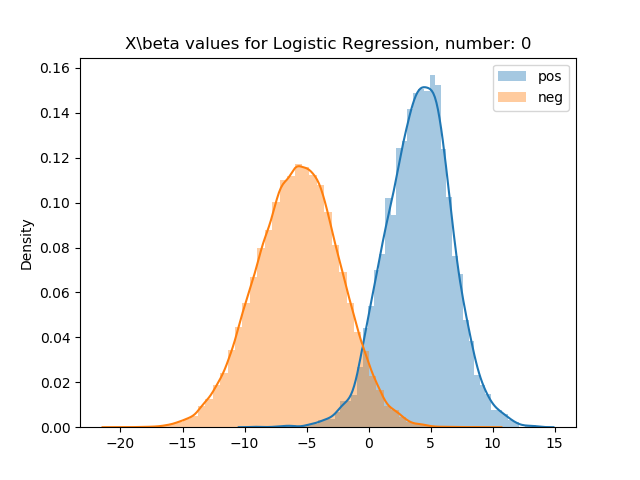
\includegraphics[width=0.95\textwidth]{fig/lr/0_weighted.png}
    \end{minipage}
    \begin{minipage}{0.19\textwidth}
        \centering
        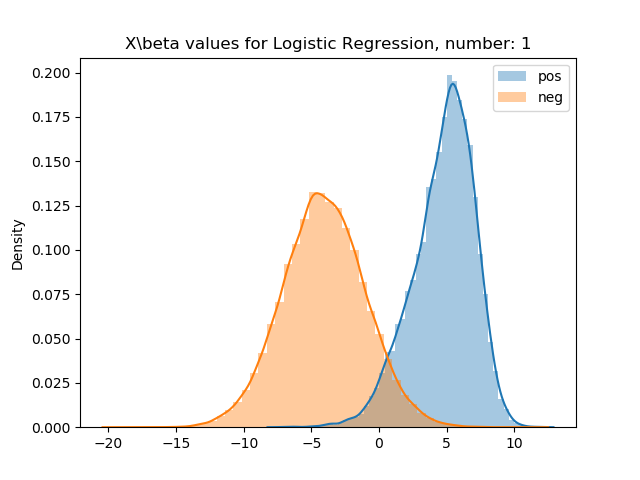
\includegraphics[width=0.95\textwidth]{fig/lr/1_weighted.png}
    \end{minipage}
    \begin{minipage}{0.19\textwidth}
        \centering
        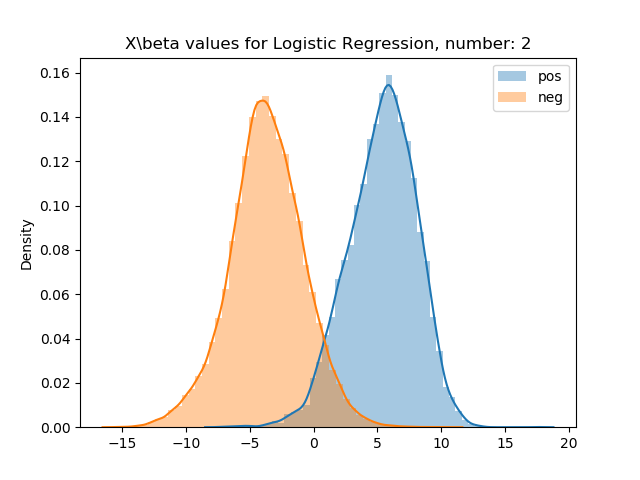
\includegraphics[width=0.95\textwidth]{fig/lr/2_weighted.png}
    \end{minipage}
    \begin{minipage}{0.19\textwidth}
        \centering
        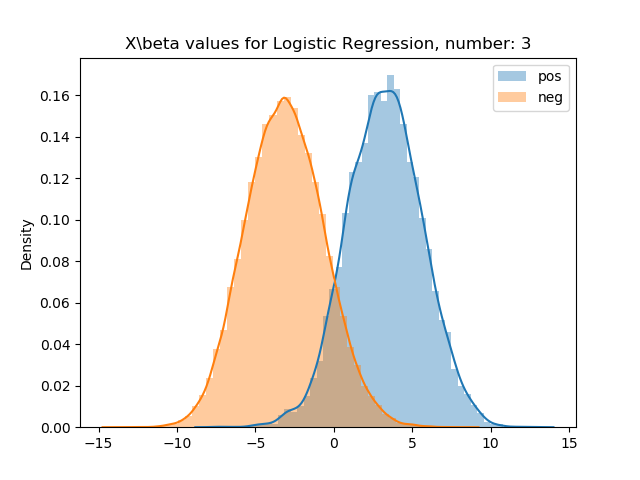
\includegraphics[width=0.95\textwidth]{fig/lr/3_weighted.png}
    \end{minipage}
    \begin{minipage}{0.19\textwidth}
        \centering
        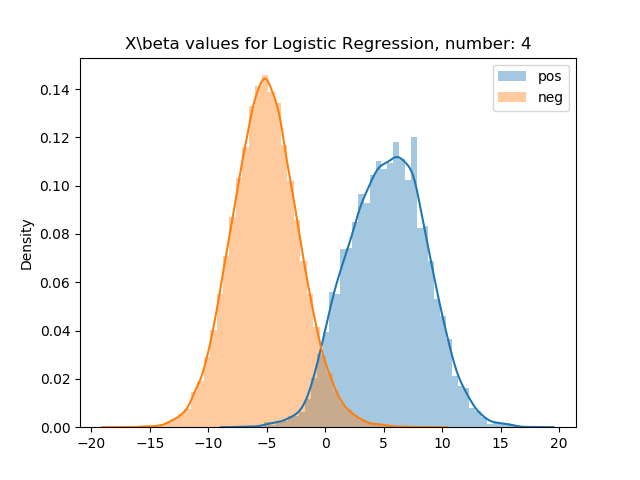
\includegraphics[width=0.95\textwidth]{fig/lr/4_weighted.png}
    \end{minipage}
    \caption{Distribution of $X^\top\beta$ for weighted LR (equivalent to sampling positive and negative samples at a ratio 1:1)}
\end{figure}
\begin{figure}[H]
    \centering
    \begin{minipage}{0.19\textwidth}
        \centering
        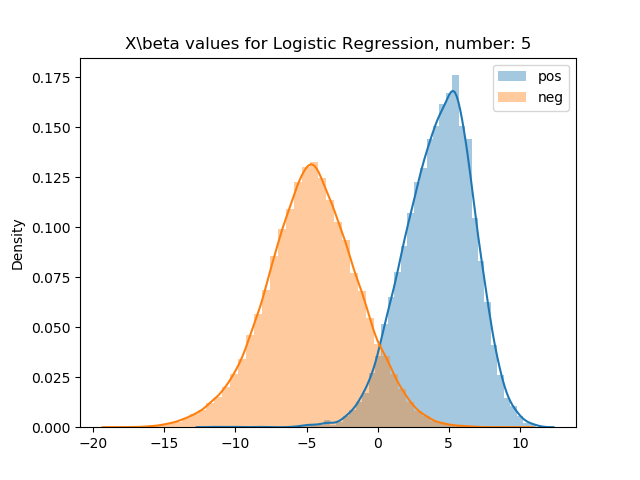
\includegraphics[width=0.95\textwidth]{fig/lr/5_weighted.png}
    \end{minipage}
    \begin{minipage}{0.19\textwidth}
        \centering
        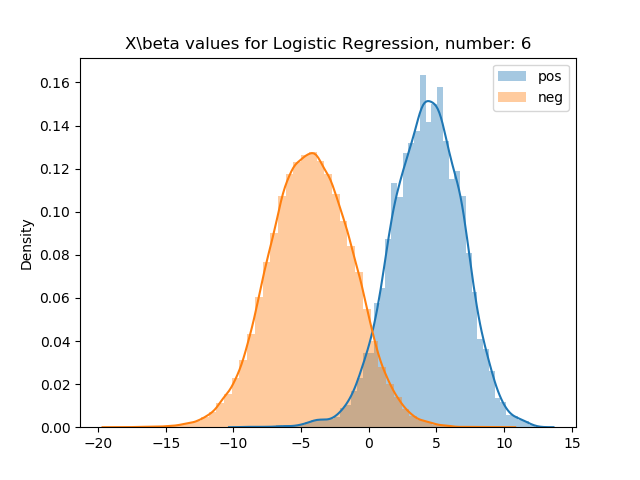
\includegraphics[width=0.95\textwidth]{fig/lr/6_weighted.png}
    \end{minipage}
    \begin{minipage}{0.19\textwidth}
        \centering
        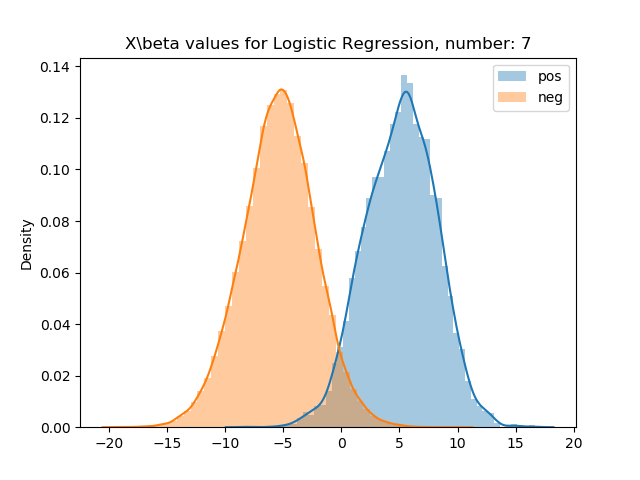
\includegraphics[width=0.95\textwidth]{fig/lr/7_weighted.png}
    \end{minipage}
    \begin{minipage}{0.19\textwidth}
        \centering
        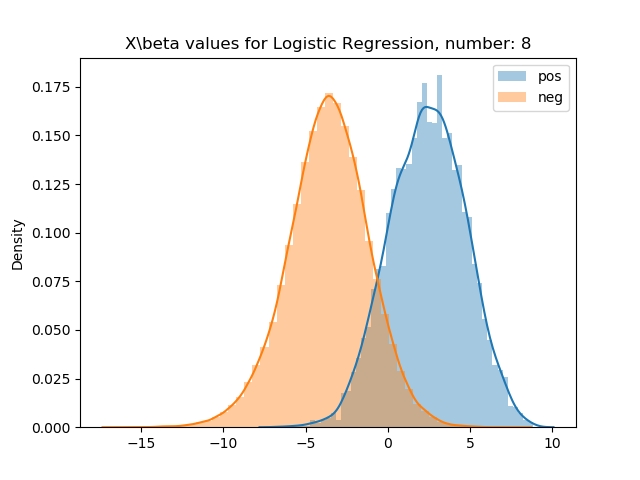
\includegraphics[width=0.95\textwidth]{fig/lr/8_weighted.png}
    \end{minipage}
    \begin{minipage}{0.19\textwidth}
        \centering
        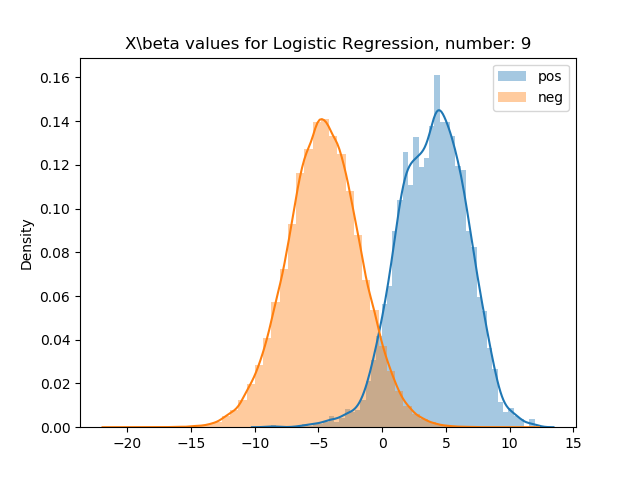
\includegraphics[width=0.95\textwidth]{fig/lr/9_weighted.png}
    \end{minipage}
    \caption{Distribution of $X^\top\beta$ for weighted LR (equivalent to sampling positive and negative samples at a ratio 1:1)}
\end{figure}

\section{Kernel Based LR}
\subsection{Implement}
All are based on $\beta=\sum_{i}\alpha_i X_i$, i.e. parameter must be the linear combination of input features. So for kernel trick, $\beta=\sum_{i}\alpha_i\phi(X_i)$. So for training, we have:
\begin{equation}
    p_i = \mathtt{sigmoid}(\phi(X_i)^\top\beta)=\mathtt{sigmoid}(K_{i,:} \alpha) 
\end{equation}
\begin{equation}
    \dfrac{\partial}{\partial \alpha}L_i = (y_i-p_i)K_{i,:}^T
\end{equation}
For prediction, it is almost the same. \\
Here I use the \textbf{rbf} kernel.
\subsection{Result}
\subsubsection{Settings}
The parameters are the same as LR. But because the kernel matrix can not be too big, so in this model, I only use the first 10000 images in the original train folder as the train set.
\subsubsection{Performance - rbf coef}
In rbf kernel, we have a hyperparameter $\sigma$, $K(X_i, X_j)=\exp\left(-\dfrac{1}{2\sigma^2}||X_i-X_j||_2^2\right)$. From my personal opinion, 
rbf kernel is just to find the data similar to the input data among the saved train data. And the measure of similarity is the rbf kernel.

In my opinion, $\sigma$ is an estimate of the size of the space that each support vector can support. A too small $\sigma$ corresponds to that each point only cares about the local space near it, which will degenerate the model into a 
look-up table, resulting in overfitting.Too large $\sigma$ corresponds to that each points supports a large piece of space, which is beyond the scope of itself, so that the similarity between the input data and the training samples can not be 
accurately measured, which will lead to under-fitting.

The results are shown in Table \ref{kernellr}.
\begin{table}[H]
    \centering
    \caption{Performance - rbf coef}
    \label{kernellr}
    \begin{tabular}{c|cc}
        \hline
        $2\sigma^2$ & Train Acc & Test Acc\\ 
        \hline
        1 & 1.0000 & 0.6917\\
        10 & 0.9847 & 0.8182\\
        100 & 0.8167 & 0.7472\\
        \hline
    \end{tabular}
\end{table}
The results are in line with my expectations, and can verify the assertion I mentioned above.\\
Kernel based LR model is better than linear LR model in terms of fitting ability, at least the latter can not even fit the train data set to 1.0000 Acc.

\section{SVM}
\subsection{Implement}
Use the third-party library sklearn.svm.SVC.\\
Use 10 independent binary SVM classifiers to do the multi-classify task.
\subsection{Result}
\subsubsection{Settings}
Train and test data set settings are the same as that of Kernel based LR model.\\
Use rbf kernel. I do not try others kernel. In the absence of sufficient theoretical support, trying many different kernel will yield little benefit. The rbf kernel is used because in the subsequent t-SNE visualization, the features appear clustered.

\subsubsection{Performance}
I tried two ways in prediction step:
\begin{itemize}
    \item SVM only output 0 or 1 as the prediction result. If there are more than one models output 1, than randomly choose one as the prediction result of multi-classify task.
    \item SVM report the decision function value, i.e. tells me the distance to the bound. Then take argmax as the result for multi-classify task. 
\end{itemize}
\begin{figure}[H]
    \centering
    \begin{minipage}{0.48\textwidth}
        \centering
        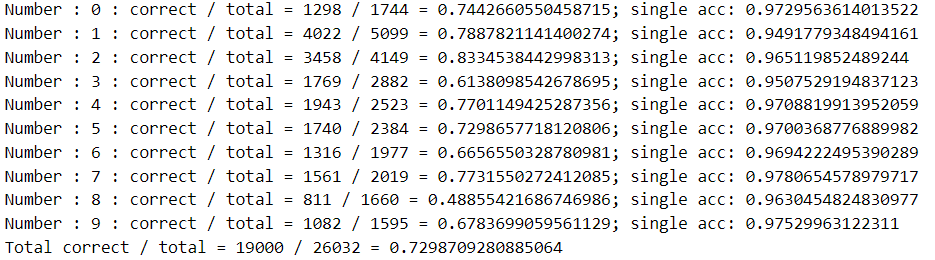
\includegraphics[width=0.95\textwidth]{fig/svm/1.png}
        report 0 or 1
    \end{minipage}
    \begin{minipage}{0.48\textwidth}
        \centering
        \includegraphics[width=0.95\textwidth]{fig/svm/2.png}
        report decision function value, i.e. tells the distance to the bound
    \end{minipage}
    \caption{SVM results}
    \label{svmresult}
\end{figure}
The results are shown in Fig. \ref{svmresult}.
\section{CNN}
\subsection{Implement}
I use a very simple toy CNN designed by myself.
\begin{table}[H]
    \centering
    \caption{CNN layers}
    \label{cnnlayers}
    \begin{tabular}{|cc|cc|}
        \hline
        Layer Number & Layer & Layer Number & Layer\\
        \hline
        1 & Conv(3, 64, 3, 2, 1) & 2 & BatchNorm + ReLU\\
        3 & Conv(64, 128, 3, 2, 1) & 4 & BatchNorm + ReLU\\
        5 & Conv(128, 256, 3, 2, 1) & 6 & BatchNorm + ReLU\\
        7 & Conv(256, 512, 3, 2, 1) & 8 & BatchNorm + ReLU\\
        9 & Conv(512, 1024, 3, 2, 1) & 10 & ReLU\\
        11 & FC(1024, 10) & 12 & Softmax\\
        \hline
    \end{tabular}
\end{table}
The network structure is shown the Table \ref{cnnlayers}. The Conv layer is given in the format Conv(input channel, output channel, kernel size, stride, padding). The FC layer is given in the format FC(input channel, output channel).
Why use kernel size = 3, stride = 2, padding = 1 ? Because in this way, the height and width of feature will reduce to half after each Conv layer. 
\subsection{Result}
\subsubsection{Settings}
The train and test data set is the same as that of LR model.\\
Use Adam optimizer provided by pytorch library. lr = 1e-3. Train for 30 epochs.\\
\subsubsection{Performance}
Overall Accuracy: 0.9015
The loss curve is shown in Fig. \ref{cnnloss}.
\begin{figure}[H]
    \centering
    \includegraphics[width=0.6\textwidth]{fig/cnn/1.png}
    \caption{CNN loss curve}
    \label{cnnloss}
\end{figure}
\subsection{Analysis}
I have not studied the nature of CNN too much. Here I just treat CNN as a learnable feature extractor + a linear multi-classifier. For linear classifier, I have discussed before. I will show the part of feature extractor in the visualization part later.
\section{Visualization of Features}
\subsection{For HOG features}
\subsubsection{PCA}
\begin{figure}[H]
    \centering
    \begin{minipage}{0.32\textwidth}
        \centering
        \includegraphics[width=0.95\textwidth]{fig/pca/0.png}
        PCA for digit 0
    \end{minipage}
    \begin{minipage}{0.32\textwidth}
        \centering
        \includegraphics[width=0.95\textwidth]{fig/pca/1.png}
        PCA for digit 1
    \end{minipage}
    \begin{minipage}{0.32\textwidth}
        \centering
        \includegraphics[width=0.95\textwidth]{fig/pca/2.png}
        PCA for digit 2
    \end{minipage}
    \includegraphics[width=0.6\textwidth]{fig/pca/pca.png}
    \caption{PCA for digits 0, 1 and 2, and t-SNE for all 10 digits}
    \label{pca012}
\end{figure}
Fig. \ref{pca012} shows the PCA visualization of HOG features for the digit 0, 1 and 2 and for all 10 digits. Seems not very linearly separable.
\subsubsection{t-SNE}
First using PCA reduce the features from 1764-dim to 100-dim, then performs t-SNE.
\begin{figure}[H]
    \centering
    \begin{minipage}{0.32\textwidth}
        \centering
        \includegraphics[width=0.95\textwidth]{fig/pca/t0.png}
        t-SNE for digit 0
    \end{minipage}
    \begin{minipage}{0.32\textwidth}
        \centering
        \includegraphics[width=0.95\textwidth]{fig/pca/t1.png}
        t-SNE for digit 1
    \end{minipage}
    \begin{minipage}{0.32\textwidth}
        \centering
        \includegraphics[width=0.95\textwidth]{fig/pca/t2.png}
        t-SNE for digit 2
    \end{minipage}
    \includegraphics[width=0.6\textwidth]{fig/pca/tsne.png}
    \caption{t-SNE for digits 0, 1 and 2, and t-SNE for all 10 digits}
    \label{tsne012}
\end{figure}
Fig. \ref{tsne012} shows the t-SNE visualization of HOG features for the digit 0, 1 and 2 and for all 10 digits. Seems suitable to solved by kernel method, especially rbf kernel.
\subsubsection{Kernel PCA}
Perform Kernel PCA to do the visualization with rbf kernel (gamma = $\dfrac{1}{2\sigma}=10$ here. This setting is from my experiment on Kernel based LR).
\begin{figure}[H]
    \centering
    \begin{minipage}{0.32\textwidth}
        \centering
        \includegraphics[width=0.95\textwidth]{fig/pca/kpca0.png}
        t-SNE for digit 0
    \end{minipage}
    \begin{minipage}{0.32\textwidth}
        \centering
        \includegraphics[width=0.95\textwidth]{fig/pca/kpca1.png}
        t-SNE for digit 1
    \end{minipage}
    \begin{minipage}{0.32\textwidth}
        \centering
        \includegraphics[width=0.95\textwidth]{fig/pca/kpca2.png}
        t-SNE for digit 2
    \end{minipage}
    \includegraphics[width=0.6\textwidth]{fig/pca/kernelpca.png}
    \caption{t-SNE for digits 0, 1 and 2, and Kernel PCA for all 10 digits}
    \label{kpca012}
\end{figure}
Fig. \ref{kpca012} shows the Kernel PCA visualization of HOG features for the digit 0, 1 and 2 and for all 10 digits. Seems much more separable than that of PCA. This may be a reason for why I use rbf kernel in this project.

\subsection{CNN Feature}
I treat CNN as a feature extractor + a classifier. So I want to know the performance of this feature extractor.\\
I visualization the features from the last layers except FC layer. The result is shown in Fig. \ref{cnnfeature}
\begin{figure}[H]
    \centering
    \begin{minipage}{0.48\textwidth}
        \centering
        \includegraphics[width=0.95\textwidth]{fig/pca/cnnpca.png}
        PCA
    \end{minipage}
    \begin{minipage}{0.48\textwidth}
        \centering
        \includegraphics[width=0.95\textwidth]{fig/pca/cnntsne.png}
        PCA to 100-dim + t-SNE
    \end{minipage}
    \caption{CNN Feature Visualization}
    \label{cnnfeature}
\end{figure}
Fig. \ref{cnnfeature} tells why the test Acc of CNN model is high. The learnable convolutional feature extractor perform much better than the manual feature extractor HOG. The features are significantly more separable. 
\section{A Naive And Immature Idea}
We have discussed in class that the error $\epsilon$ of the regression model should be uncorrelated to $X^\top\beta$, i.e. $\mathbb{E}[\epsilon_iX_i^\top\beta]=\mathbb{E}[\epsilon_i]\mathbb{E}[X_i^\top\beta]=0$. I want to check this assertion in logistic regression model. \\

In the logistic regression $\epsilon_i = y_i - p_i$. From the gradient $\partial L/\partial\theta = \sum_{i} (y_i-p_i)X_i = \sum_{i} X_i\cdot \epsilon_i$, I found that $\mathbb{E}[\beta^\top X_i^\top \epsilon_i]=\mathtt{const}\cdot \beta^\top \nabla_\theta L = 0$ as long as the model is optimal.\\

However, if performing Ridge regression (with a coef $\lambda$), $\mathbb{E}[\epsilon_i X^\top_i\beta] \propto \lambda \beta^\top\beta > 0$ when the model is optimal.  \\

I calculate the $\mathbb{E}[\epsilon_i X^\top_i\beta]$ value according to the result from my LR model and LR + Ridge model. The results are shown in Table \ref{error}.
\begin{table}[H]
    \centering
    \caption{Error - Ridge}
    \label{error}
    \begin{tabular}{c|c}
        \hline
        $\lambda$ & $\mathbb{E}[\epsilon_i X_i^\top\beta]$\\
        \hline
        $0$ & $-1.565\times 10^{-4}$\\
        $0.1$ & $3.756\times 10^{-2}$\\
        $0.01$ & $5.367\times 10^{-3}$\\
        \hline        
    \end{tabular}
\end{table}
The result shows that without Ridge loss, the error is really uncorrelated to the input. But with Ridge loss, the error is a little positive correlated to the projected input $X^\top\beta$.

But for this characteristic of Ridge regression, I have not come up with a reasonable explanation.
\section{The End}
I have implemented several typical ML model in this project. For LR, LDA and Kernel LR, I have given some intuitive or theoretical analysis. For all the models, I have performed experiments to make sure that they work. And I have shown the visualization result for the HOG feature. 

The most interesting analysis, I think, is about the distribution of $X^\top\beta$, and I explanation the relationship between the distribution and the sigmoid / logistic function, and then provide a reasonable explanation for logistic regression method.

\end{document}
